\documentclass[a4,12pt]{horizon-theme}
\usepackage{lipsum}
\usepackage{fontawesome5}
\usepackage{graphicx,url}
\usepackage{float}
\usepackage{amsmath}
\usepackage{booktabs}
\usepackage{makecell}
\usepackage{array}
\usepackage{multirow}
\usepackage{caption}
\usepackage{subcaption}
\usepackage{siunitx}
\usepackage{enumerate}
\usepackage{gensymb}
\usepackage{csvsimple}
% \usepackage{tabularray}
\usepackage{stackengine}
\usepackage{xcolor, colortbl}
\usepackage[round]{natbib}
\usepackage{karnaugh-map}
\usepackage{stackengine}
% \usepackage{longtable}
\usepackage{minted}

\strutlongstacks{T}

\BeforeBeginEnvironment{minted}{\vspace{-20pt}}


% Cover Config
% \configCover{<num. do exp.>}{<data>}{<título>}
\configCover{5}{26/05/2022}{Projeto de Circuitos Digitais em VHDL}



\begin{filecontents*}{tb_testes.csv}
clock,zera,vagas,conta,direcao,contagem,cheio
$\times$,1,$\times$,$\times$,$\times$,000,0
$\uparrow$,0,110,1,1,001,0
$\uparrow$,0,110,1,1,010,0
$\uparrow$,0,110,1,1,011,0
$\uparrow$,0,110,1,1,100,0
$\uparrow$,0,110,1,1,101,0
$\uparrow$,0,110,1,1,110,1
$\uparrow$,0,110,1,0,110,1
$\uparrow$,0,110,1,0,101,0
$\uparrow$,0,110,1,0,100,0
$\uparrow$,0,110,1,0,011,0
$\uparrow$,0,110,1,0,010,0
$\uparrow$,0,110,1,0,001,0
$\uparrow$,0,110,1,0,000,0
\end{filecontents*}



\newenvironment{code}{\captionsetup{type=listing}}{}


\begin{document}
\horizonCover

\horizonTitle


\section{Introdução} % R
O VHDL é uma linguagem de descrição de hardware. Com ela é possível descrever e simular circuitos digitais dos mais diversos sem a necessidade de se montar o circuito e testá-lo a cada alteração na descrição. Nesse experimento, será realizado um projeto simples utilizadno o VHDL.

\section{Objetivos} % N
O objetivo deste experimento é desenvolver o projeto de um comparador, um contador direcional e outro bidirecional usando VHDL sob o paradígma comportamental e usar os componentes menores para desenvolver um projeto de controle de vagas de estacionamento usando VHDL sob o paradígma estrutural.


\section{Planejamento} % N, R
\label{sec:plan}

\subsection{Comparador e Contador em VHDL}
\label{sec:plan_1}

\subsubsection{Implementação}
\label{sec:plan_1_impl}
Os cirucitos forma implementados em VHDL usando o paradigma comportamental. A descrição comentada do circuito comparador está disposta na Listagem \ref{lst:comparador} e a descrição do circuito contador está na Listagem \ref{lst:contador} no Apêndice \ref{ap:vhdl}.


\subsubsection{Simulação}
\label{sec:plan_1_sim}

As cartas dos tempos do circuito comparador e comparador estão dispostas nas Figs. \ref{fig:ct_comparador} e \ref{fig:ct_contador}, respectivamente.

\begin{figure}[!ht]
  \centering
  \includegraphics[width=\textwidth]{comparador.png}
  \caption{Carta dos tempos para o circuito comparador}
  \label{fig:ct_comparador}
\end{figure}


\begin{figure}[!ht]
  \centering
  \includegraphics[width=\textwidth]{contador.png}
  \caption{Carta dos tempos para o circuito contador}
  \label{fig:ct_contador}
\end{figure}


\subsubsection{Contador Bidirecional}
\label{sec:plan_1_ud}
Foi adicionado um novo sinal de entrada denominado ``direção'', que controla o comportamento da contagem. A contagem é crescente caso esse sinal seja alto e descrescente caso contrário. Com essa modificação foi implementado um circuito contador bidirecional $\textrm{UP/}\n{\textrm{DOWN}}$. A Listagem \ref{lst:contador_ud} mostra a descrição deste circuito e a Fig. \ref{fig:ct_contador_ud} mostra a carta dos tempos.

\begin{figure}[!ht]
  \centering
  \includegraphics[width=\textwidth]{contador_ud.png}
  \caption{Carta dos tempos do circuito contador bidirecional}
  \label{fig:ct_contador_ud}
\end{figure}

\newpage
\subsection{Controle de Vagas de Estacionamento}
\subsubsection{Implementação}

De modo a atender a necessidade de um contagem acíclica e bidirecional para o projeto do controle de vagas de estacionamento, a descrição do contador bidirecional (\ref{lst:contador_ud}) foi alterada de modo a limitar a contagem de 0 a 15 de forma acíclica. Essa nova descrição se encontra na Listagem \ref{lst:contador_acíclico}.

\begin{code}
  \captionof{listing}{Descrição do circuito contador bidirecional acíclico de 4 bits.}
  \label{lst:contador_acíclico}
  \begin{minted}[frame=lines, framesep=6pt, framerule=0.5pt, linenos, rulecolor=secondaryColor]{VHDL}
-- contador.vhd
-- contador bidirecional acíclico de 4 bits

library IEEE;
use IEEE.std_logic_1164.all;
use IEEE.numeric_std.all;

entity contador is
  port (
    clock, zera, conta, direcao: in std_logic;
    contagem: out std_logic_vector(3 downto 0)
  );
end contador;

architecture contador_arch of contador is
  signal IQ: integer range 0 to 15;
begin
  process(clock, zera, conta)
  begin
    if zera='1' then
      IQ <= 0;
    elsif clock'event and clock='1' then    
      if conta='1'then
			if (direcao='1' and IQ<15) then
				IQ <= IQ + 1;
			elsif (direcao='0' and IQ>0) then
				IQ <= IQ - 1;
			end if;
		else
			IQ <= IQ;
		end if;
	 end if;
  end process;
  contagem <= std_logic_vector(to_unsigned(IQ, contagem'length));
end contador_arch;
\end{minted}
\end{code}

Além disso também foram implementadas a descrição do sinalizador de vagas e a descrição estrutural da integração desses dois circuitos, ambos podem ser vistos nas Listagens \ref{lst:sinalizador} e \ref{lst:controle}.

\begin{code}
  \captionof{listing}{Descrição do circuito Sinalizador de Vagas.}
  \label{lst:sinalizador}
  \begin{minted}[frame=lines, framesep=6pt, framerule=0.5pt, linenos, rulecolor=secondaryColor]{VHDL}
-- sinalizador.vhd
-- sinalizador de vagas

library IEEE;
use IEEE.std_logic_1164.all;
use IEEE.numeric_std.all;

entity sinalizador is
  port (
    vagas, contagem: in std_logic_vector(3 downto 0);
    fim: out std_logic
  );
end sinalizador;

architecture sinalizador_arch of sinalizador is
  begin
  
	fim <= '0' when vagas>contagem else '1';

end sinalizador_arch;
\end{minted}
\end{code}

\begin{code}
  \captionof{listing}{Descrição estrutural de um Controle de Vagas de Estacionamento.}
  \label{lst:controle}
  \begin{minted}[frame=lines, framesep=6pt, framerule=0.5pt, linenos, rulecolor=secondaryColor]{VHDL}
-- controle.vhd
-- controle de vagas de estacionamento

library IEEE;
use IEEE.std_logic_1164.all;
use IEEE.numeric_std.all;

entity controle is
  port (
    clock, zera, conta, direcao: in std_logic;
	 vagas: in std_logic_vector(3 downto 0);
	 contagem: out std_logic_vector(3 downto 0);
	 cheio: out std_logic
  );
end controle;

architecture controle_arch of controle is

	component contador is
	  port (
		 clock, zera, conta, direcao: in std_logic;
		 contagem: out std_logic_vector(3 downto 0)
	  );
	end component;
	
	component sinalizador is
	  port (
		 vagas, contagem: in std_logic_vector(3 downto 0);
		 fim: out std_logic
	  );
	end component;
	
	signal quant_vagas: std_logic_vector(3 downto 0);

begin
	contagem <= quant_vagas;
	contador_1: contador port map (clock, zera, conta, direcao, quant_vagas);
	sinalizador_1: sinalizador port map (vagas, quant_vagas, cheio);
end controle_arch;
\end{minted}
\end{code}

\newpage
\subsubsection{Diagrama de blocos}

O diagrama de blocos obtido com a função RTL Viewer da ferramenta Quartus na Figura \ref{fig:diagrama_blocos}.

\begin{figure}[!ht]
  \centering
  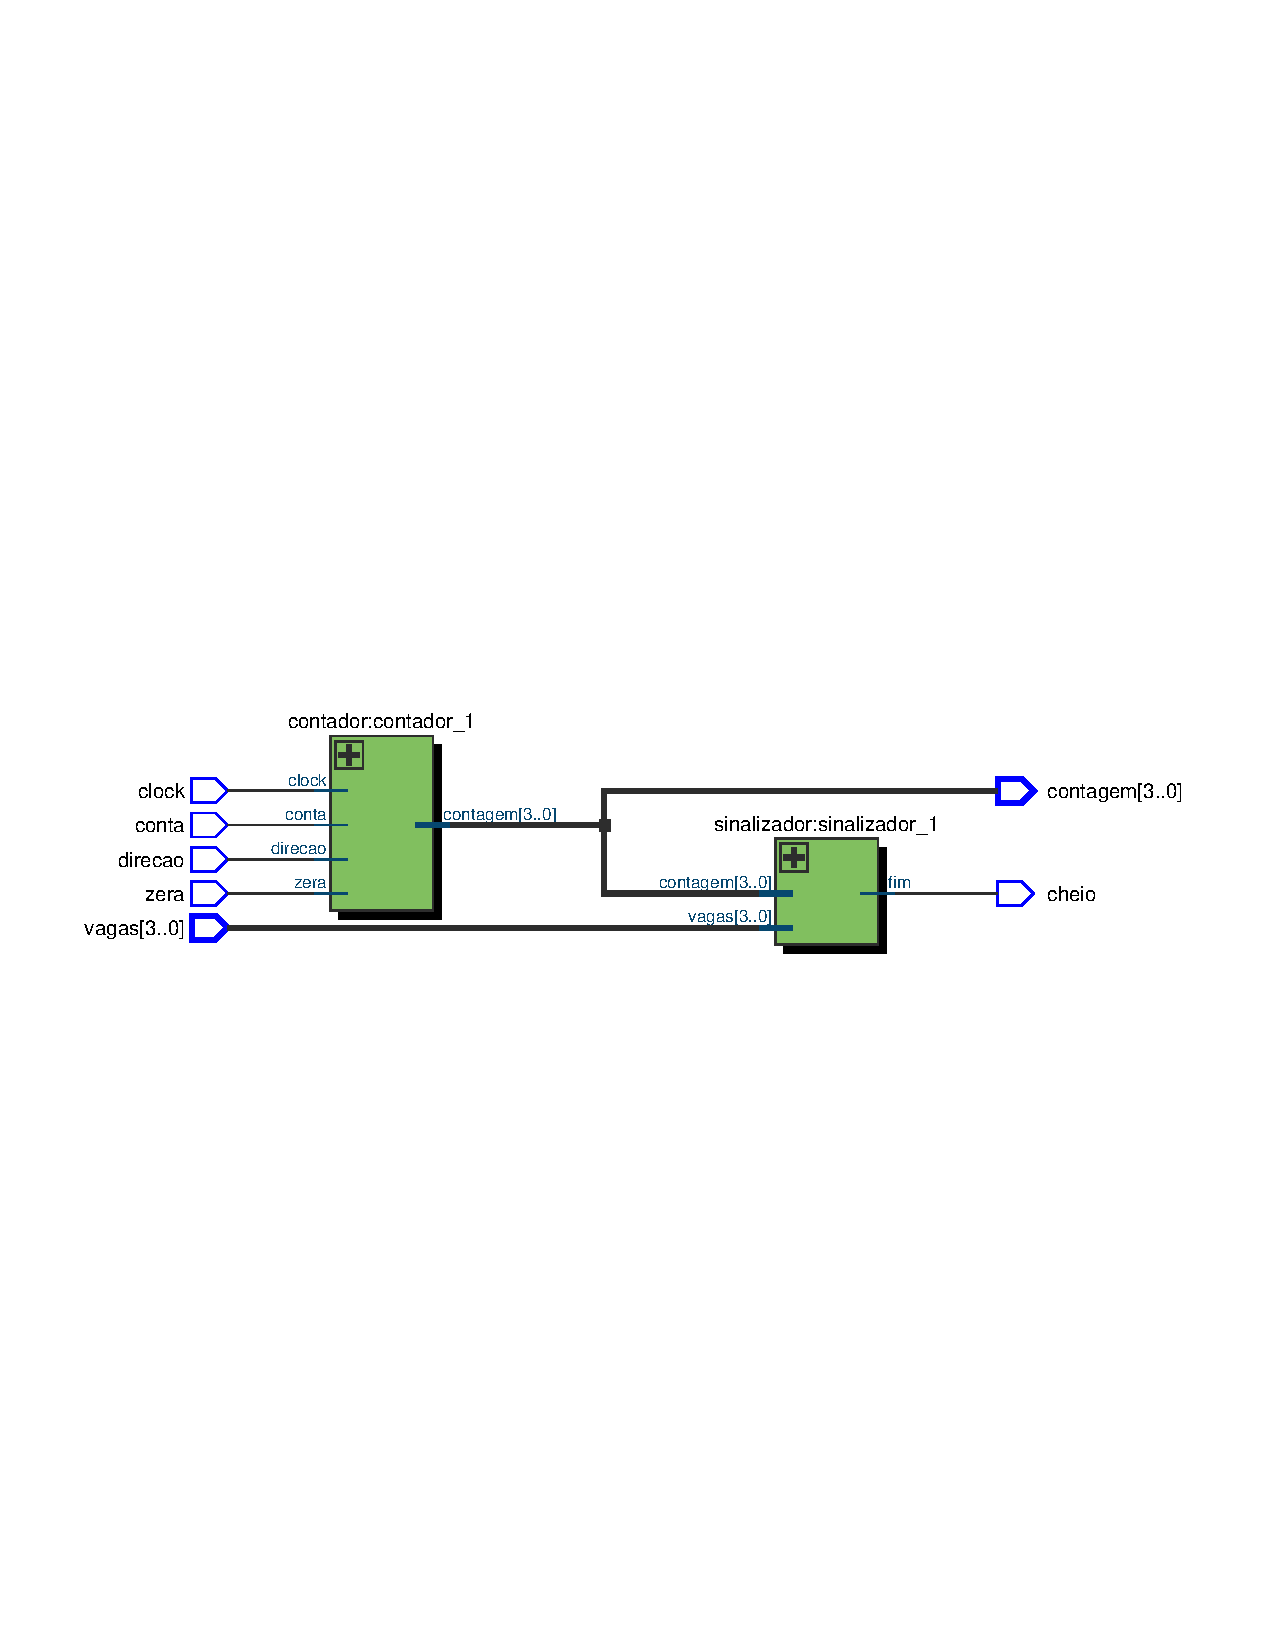
\includegraphics[width=\textwidth, trim={5mm, 110mm, 5mm, 110mm}, clip]{diagrama.pdf}
  \caption{Diagrama de blocos do Controle de Vagas de Estacionamento}
  \label{fig:diagrama_blocos}
\end{figure}

O sinal de saída ``contagem'' foi utilizado apenas para facilitar a depuração.

\subsubsection{Simulação}

A carta de tempos que simula o funcionamento do circuito pode ser vista na Figura \ref{fig:carta_controle}. Para essa simulação tentou-se imitar uma situação na qual o número máximo de vagas é 6 e entram carros até encher o estacionamento e depois esses carros saem até esvaziá-lo.

\begin{figure}[!ht]
  \centering
  \includegraphics[width=\textwidth]{carta_controle.png}
  \caption{Carta de tempos da simulação do circuito Controle de Vagas de Estacionamento.}
  \label{fig:carta_controle}
\end{figure}


\newpage
\subsubsection{Tabela de testes}
A Tabela \ref{tab:testes} motra a Tabela de Testes do circuito de controle de vagas

\begin{table}[!ht]
  \centering
  \caption{Tabela de testes do circuito de controle de vagas}
  \label{tab:testes}
  \doubleRuleSep
  \begin{tabular}{*{7}{c}}
    \doubleTopRule
    \multicolumn{5}{c}{Entradas} & Depuração & Saída                                                       \\
    \cmidrule(lr){1-5}\cmidrule(lr){6-6}\cmidrule(lr){7-7}
    clk                          & zera      & vagas      & conta     & direcao  & contagem  & cheio       \\
    \midrule
    \csvreader[head to column names, late after line=\\]{tb_testes.csv}{}%
    {\csvcoli                    & \csvcolii & \csvcoliii & \csvcoliv & \csvcolv & \csvcolvi & \csvcolvii} %
    \doubleBottomRule
  \end{tabular}
\end{table}



\section{Resultados}
O sistema digital planejado foi implantado na placa FPGA com sucesso. O circuito apresentou o comportamento desejado para todos os testes e nenhuma alteração do projeto foi necessária. Adicionalmente, foi feita uma modificação do projeto para que o contador parasse a contagem assim que atingisse o valor máximo de vagas.




\section{Desafio}
Foi incluído um novo sinal de entrada no circuito contador de vagas de estacionamento que, quando em nível lógico alto, modifica o contador para incrementar/decrementar de duas unidades, ao invés de uma, e, quando em nível lógico baixo, não modifica nenhum comportamento do circuito, ou seja, continua contado de um em um.

As Listagens \ref{lst:desafio_contador} e \ref{lst:desafio_controle} mostram as diferenças entre as descrições anteriores (\ref{lst:contador_acíclico} e \ref{lst:controle}) e as atuais para os componentes \texttt{contador} e \texttt{controle}, respectivamente, e o componente \texttt{sinalizador} não foi alterado. A Fig. \ref{fig:desafio} mostra o diagrama de blocos do novo circuito, alterações incluem o recebimento do sinal \texttt{duplo} e a realimentação do sinal \texttt{cheio} no contador.

Após a montagem, o circuito apresentou todos os comportamentos esperados.

\begin{figure}[!ht]
  \centering
  \includegraphics[width=\textwidth, trim={25mm, 100mm, 25mm, 108mm}, clip]{desafio.pdf}
  \caption{Diagrama de blocos do circuito considerando contagem dupla}
  \label{fig:desafio}
\end{figure}



\section{Conclusão}
Com este experimento, pudemos projetar, simular e implantar um circuito digital para controle de vagas em um estacionamento em uma placa FPGA. A descrição deste circuito foi feita explorando dois paradígmas do VHDL: o comportamental, usado para descrever os componentes menores, e o estrutural, usado para unir os componentes do circuito. Durante a implantação não houve nenhuma alteração do planejamento e o circuito operou como planejado.



\newpage
\appendix
\section*{Apêndice}
\renewcommand{\thesubsection}{\Alph{subsection}}

\subsection{Descrições dos circuitos}
\label{ap:vhdl}

Descrições comentadas dos circuitos comparador e contador em VHDL

\begin{code}
  \captionof{listing}{Descrição do circuito comparador}
  \label{lst:comparador}
  \begin{minted}[frame=lines, framesep=6pt, framerule=0.5pt, linenos, rulecolor=secondaryColor]{VHDL}
-- comparador.vhd
-- comparador binario com entradas de 2 bits

library IEEE;
use IEEE.std_logic_1164.all;

-- definição das portas de entrada e saída
entity comparador is
  port (
    A, B: in std_logic_vector(1 downto 0);
    igual: out std_logic
  );
end comparador;

-- descrição das ligações internas do circuito
architecture comportamental of comparador is
begin
  -- o sinal igual terá nível lógico alto sempre que os sinais A e B
  -- tiverem o mesmo nível lógico, caso contrário terá nível lógico baixo
  igual <= '1' when A=B else '0';
end comportamental;
\end{minted}
\end{code}


\newpage
\begin{code}
  \captionof{listing}{Descrição do circuito contador}
  \label{lst:contador}
  \begin{minted}[frame=lines, framesep=6pt, framerule=0.5pt, linenos, rulecolor=secondaryColor]{VHDL}
-- contador.vhd
-- contador hexadecimal de 4 bits

library IEEE;
use IEEE.std_logic_1164.all;
use IEEE.numeric_std.all;

-- definição dos sinais de entrada e saída do circuito
entity contador is
  port (
    clock, zera, conta, carrega: in std_logic;
    entrada: in std_logic_vector(3 downto 0);
    contagem: out std_logic_vector(3 downto 0);
    fim: out std_logic
  );
end contador;


-- implementação comportamental do circuito contador
architecture comportamental of contador is
  -- sinal IQ: sinal do tipo inteiro que armazena o valor atual do contador
  signal IQ: integer range 0 to 15;
begin
  process(clock, zera, conta, carrega, entrada, IQ)
  -- define um processo sensível à mudança dos níveis lógicos dos sinais
  -- clock, zera, conta, carrega, entrada e IQ
  -- os sinais zera, conta e carrega definem as ações do circuito
  begin
    if zera='1' then
      -- clear assíncrono (não depende da borda de subida do clock)
      IQ <= 0; -- zera o valor do contador
    
    elsif clock'event and clock='1' then
      -- ações sensíveis à borda de subida do clock são colocadas aqui
      -- há duas ações possíveis: carregar os dados (maior precedência) 
      -- e incrementar o valor do sinal em 1 (menor precedência)
      -- apenas uma das ações é performada por clock
      
      if carrega='1' then
        -- ação "carrega": configura o contador para receber 
        -- um valor específico de um sinal de entrada do circuito
        IQ <= to_integer(unsigned(entrada));
      
      elsif conta='1' then  
        -- ação "conta": lógica de um acumulador circular, 
        -- incrementa o valor atual em 1 se o valor atual for menor 
        -- que o valor máximo, zera caso contrário
        if IQ=15 then 
          IQ <= 0;
        else 
          IQ <= IQ + 1;
        end if;
      
      else
        -- se nenhuma ação for especificada, o contador permanece com
        -- o sinal atual
        IQ <= IQ;
      end if;
    end if;
  end process;

  -- liga do sinal interno IQ ao sinal de saída do contador
  -- faz cast de inteiro para std_logic_vector
  contagem <= std_logic_vector(to_unsigned(IQ, contagem'length));

  -- detecta quando o contador atinge o valor máximo
  fim <= '1' when IQ=15 else '0';
end comportamental;
\end{minted}
\end{code}


\newpage
\begin{code}
  \captionof{listing}{Descrição do circuito contador $\textrm{UP/}\n{\textrm{DOWN}}$. Os comentários no código foram omitidos, já que as modificações estão comentadas na Seção \ref{sec:plan_1_ud}}
  \label{lst:contador_ud}
  \begin{minted}[frame=lines, framesep=6pt, framerule=0.5pt, linenos, rulecolor=secondaryColor]{VHDL}
-- contador_ud.vhd
-- contador hexadecimal bidirecional de 4 bits

library IEEE;
use IEEE.std_logic_1164.all;
use IEEE.numeric_std.all;


entity contador_ud is
  port (
    clock, zera, conta, carrega, direcao: in std_logic;
    entrada: in std_logic_vector(3 downto 0);
    contagem: out std_logic_vector(3 downto 0);
    fim: out std_logic
  );
end contador_ud;


architecture comportamental of contador_ud is
  signal IQ: integer range 0 to 15;
begin
  process(clock, zera, conta, carrega, direcao, entrada, IQ)
  begin
    if zera='1' then
      IQ <= 0;
    elsif clock'event and clock='1' then    
      if carrega='1' then
      IQ <= to_integer(unsigned(entrada));
      elsif conta='1' then  
        if direcao='1' then
          if IQ=15 then 
            IQ <= 0;
          else 
            IQ <= IQ + 1;
          end if;
        else
          if IQ=0 then
            IQ <= 15;
          else
            IQ <= IQ - 1;
          end if;
        end if;
      else
        IQ <= IQ;
      end if;
    end if;
  end process;

  contagem <= std_logic_vector(to_unsigned(IQ, contagem'length));
  fim <= '1' when IQ=15 else '0';
end comportamental;
\end{minted}
\end{code}


\newpage
\begin{code}
  \captionof{listing}[]{Alterações na descrição do componente \texttt{controle.vhd} para implementação da contagem dupla\footnotemark}
  \label{lst:desafio_controle}
  \begin{minted}[frame=lines, framesep=6pt, framerule=0.5pt, linenos, rulecolor=secondaryColor, tabsize=2]{diff}
@@ -7,7 +7,7 @@
 
 entity controle is
   port (
-    clock, zera, conta, direcao: in std_logic;
+    clock, zera, conta, direcao, duplo: in std_logic;
     vagas: in std_logic_vector(3 downto 0);
     contagem: out std_logic_vector(3 downto 0);
     cheio: out std_logic
@@ -18,7 +18,8 @@
 
   component contador is
     port (
-      clock, zera, conta, direcao: in std_logic;
+      clock, zera, conta, direcao, cheio, duplo: in std_logic;
+      vagas: in std_logic_vector(3 downto 0);
       contagem: out std_logic_vector(3 downto 0)
     );
   end component;
@@ -31,9 +32,12 @@
   end component;
   
   signal quant_vagas: std_logic_vector(3 downto 0);
+  signal re_conta, re_cheio: std_logic;
 
 begin
   contagem <= quant_vagas;
-  contador_1: contador port map (clock, zera, conta, direcao, quant_vagas);
-  sinalizador_1: sinalizador port map (vagas, quant_vagas, cheio);
+  cheio <= re_cheio;
+  contador_1: contador port map (clock, zera, conta, direcao, re_cheio, 
+    duplo, vagas, quant_vagas);
+  sinalizador_1: sinalizador port map (vagas, quant_vagas, re_cheio);
 end controle_arch;
\end{minted}
\end{code}

\footnotetext{Gerado com \texttt{diff -Naru  controle\_vagas/controle.vhd desafio/controle.vhd}}



\newpage
\begin{code}
  \captionof{listing}[]{Alterações na descrição do componente \texttt{contador.vhd} para implementação da contagem dupla\footnotemark}
  \label{lst:desafio_contador}
  \begin{minted}[frame=lines, framesep=6pt, framerule=0.5pt, linenos, rulecolor=secondaryColor, tabsize=2]{diff}
@@ -8,25 +8,35 @@
 
 entity contador is
   port (
-    clock, zera, conta, direcao: in std_logic;
+    clock, zera, conta, direcao, cheio, duplo: in std_logic;
+    vagas: in std_logic_vector(3 downto 0);
     contagem: out std_logic_vector(3 downto 0)
   );
 end contador;
 
 
 architecture contador_arch of contador is
-  signal IQ: integer range 0 to 15;
+  signal IQ, int_vagas: integer range 0 to 15;
 begin
+  int_vagas <= to_integer(unsigned(vagas));
   process(clock, zera, conta)
   begin
     if zera='1' then
       IQ <= 0;
     elsif clock'event and clock='1' then    
       if conta='1'then
-        if (direcao='1' and IQ<15) then
-          IQ <= IQ + 1;
-        elsif (direcao='0' and IQ>0) then
-          IQ <= IQ - 1;
+        if duplo='0' then
+          if (direcao='1' and IQ<15 and cheio='0') then
+            IQ <= IQ + 1;
+          elsif (direcao='0' and IQ>0) then
+            IQ <= IQ - 1;
+          end if;
+        else
+          if (direcao='1' and IQ<(int_vagas-1) and cheio='0') then
+            IQ <= IQ + 2;
+          elsif (direcao='0' and IQ>1) then
+            IQ <= IQ - 2;
+          end if;
         end if;
       else
         IQ <= IQ;
\end{minted}
\end{code}

\footnotetext{Gerado com \texttt{diff -Naru  controle\_vagas/contador.vhd desafio/contador.vhd}}




% \bibliographystyle{plainnat}
% \bibliography{refs}

\horizonBackCover
\end{document}
